\section{Experiments}
\label{sec:Chapter_V}

This section measures the gains of the closed loop and of reservation-table-aware dispatching and whether they amplify each other, asks on which instances they hold and whether the present seeds can resolve this, and explains why the other interfaces yield no net gain.

\subsection{Experimental setup}
\label{sec:instances}

\subsubsection{Controlled instance families}
FJSP\_PT benchmarks write travel times as a matrix and supply no corridor network.
Of the \PubNLayout{} layouts of Homayouni and Fontes~\cite{homayouni2021production}, \PubNLayoutAsym{} matrices are entirely asymmetric, ruling out undirected corridors, and \PubNLayoutBad{} also violate the triangle inequality, which no graph's shortest paths do; a network reverse-engineered from them would be a different instance.
We therefore generate controlled instances on an explicit road network, so that each feature of Section~\ref{sec:features} can be varied on its own; public instances, with contention removed, calibrate only the upper-level search (Section~\ref{sec:external}).

All instances share the core of Table~\ref{tab:instances}, with $\bar{T}_t/\bar{T}_p$ scaled so that vehicle contention is the main constraint and $H$ standardized per operation so that $F$ does not change it.

\emph{Family A: layout.}
In a spine layout a main corridor (the spine) runs through the arm area and each arm hangs off it on its own branch corridor, as in high-volume plants where congestion on the central corridor is a known problem~\cite{suh2022spine}.
Placing $v_0$ at one end of the spine, rather than where trips are balanced as real shops do, sends every transport through the same exit and corridor stretch: a deliberately high-contention construction, and exactly the case the closed loop targets.
Parallel lanes of equal duration change capacity, not distance; a tandem single-vehicle loop~\cite{rahimikelarijani2020tandem} has almost no contention.
\texttt{funnel}, \texttt{high}, and \texttt{mid} differ only in their lanes; \texttt{funnel} and \texttt{high} differ by one exit at $v_0$, halving the minimum cut, a single-factor contrast.
The grids \texttt{low} and \texttt{scatter} (arms at the farthest points) cover the low-contention range, but their farthest unimpeded trip is \LegGrid{} against \LegDumbbell{}, so only differences among the spine instances are attributable to capacity.
Contention intensity (\ContentionAHi{} to \ContentionLo{}) is not monotone in this order; the paper-wide maximum \ContentionHi{} is the $F=1.0$ instance of Family~C.

\emph{Family B} varies the vehicle-to-arm ratio on \texttt{funnel} to test whether dispatching has an upper limit in fleet size; \emph{Family C} varies flexibility, the fraction of arms each operation may use.
Their shared base point \texttt{A funnel} is run once, so $5+3+2=\NCases$, and must be counted when reading Families~B and~C.
Contention intensity is measured on the initial random population because optimized solutions route around congestion and erase the differences among instances.
Relative to the \PubNInst{} public instances, our base $F$ is about one and a half times the median \PubFMed{}, $H$ exceeds the maximum \PubHMax{} (median \PubHMed{}), and $\bar{T}_t/\bar{T}_p$ deliberately exceeds the maximum \PubTtTpHi{}; whether the high $H$ inflates the closed-loop gain is tested in Section~\ref{sec:whichcongestion}.

\begin{table}[t]
\caption{Controlled instances. Shared core: $12$ jobs, $36$ real operations, $8$ arms, $H=0.3$, $\bar{T}_t/\bar{T}_p\approx4.0$.
Contention intensity: share of yielding wait in travel time on the initial random population.}
\label{tab:instances}
\small
%% 由 tab/gen_tables_ladder.py 生成:结构列直接由 tools/abc_matrix.py 的 build() 构造出
%% 算例后读出,下界调 algorithm/instance.py 的 simple_lower_bound,争用强度取自
%% baseline_ladder.csv 的 contention 列。任何一列都不是手打的。
%% 由 tab/gen_tables_ladder.py 生成,请勿手工编辑
%% 数据源:clbs/output/baseline_ladder.csv 等,见脚本首部
\begin{tabular}{@{}llrrrrrr@{}}
\toprule
Instance & Varied factor & Nodes & Corridors & $N_A$ & $F$ & Contention & Composite LB (time units) \\
\midrule
A funnel & layout & 13 & 12 & 12 & 0.61 & 31.9\% & 24.0 \\
A high & layout & 14 & 14 & 12 & 0.61 & 30.9\% & 17.0 \\
A low & layout & 16 & 24 & 12 & 0.61 & 11.8\% & 36.0 \\
A mid & layout & 15 & 16 & 12 & 0.61 & 10.8\% & 17.0 \\
A scatter & layout & 16 & 24 & 12 & 0.61 & 6.6\% & 36.0 \\
\midrule
B NA/NM 0.5 & $N_A/N_M$ & 13 & 12 & 4 & 0.61 & 15.8\% & 24.0 \\
B NA/NM 1.0 & $N_A/N_M$ & 13 & 12 & 8 & 0.61 & 30.2\% & 24.0 \\
B NA/NM 2.0 & $N_A/N_M$ & 13 & 12 & 16 & 0.61 & 32.4\% & 24.0 \\
\midrule
C F=0.3 & flexibility & 13 & 12 & 12 & 0.30 & 27.7\% & 24.0 \\
C F=1.0 & flexibility & 13 & 12 & 12 & 1.00 & 33.5\% & 24.0 \\
\bottomrule
\end{tabular}

\end{table}

\subsubsection{Comparison protocol}
\label{sec:protocol}

Every schedule is executed by the same conflict-free router and checked against the composite lower bound by a validator independent of the decoder; failing runs are reported separately.
We compare realized makespans, because the open loop's self-reported makespan is often infeasible; the gap (hereafter, the optimism margin) is especially large on the funnel layout.
One evaluation costs up to about two orders of magnitude more in some configurations than in others, so configurations share an equal wall-clock budget (Table~\ref{tab:batches}) rather than a generation count, with early stopping after $400$ generations without improvement.
Every open-loop run stops early, using about one fifth of the budget, while both closed-loop configurations use all of it; this favours the baseline, which completes as many evaluations as closed-loop rule-based dispatching, or more (Section~\ref{sec:costlaw}).

\begin{table}[t]
\caption{Experiment batches; only the main batch supports Tables~\ref{tab:main} and~\ref{tab:bytag}. Speed-ups: pruning and winner-path reuse (Section~\ref{sec:speedup}).}
\label{tab:batches}
\footnotesize
\begin{tabular}{@{}p{1.7cm}p{2.3cm}p{1.9cm}cp{1.6cm}c@{}}
\toprule
Batch & Purpose & Instances & Seeds & Wall-clock budget & Speed-ups \\
\midrule
Main & Ladder (Tables~\ref{tab:main}, \ref{tab:bytag}) & Ten controlled & $\NSeeds$ & $90$\,s & yes \\
Cost diagnosis & Figure~\ref{fig:protocol} & Three controlled & $3$ & $90$\,s & yes \\
Convergence diagnosis & Optimism margin (Section~\ref{sec:main}) & \texttt{funnel} & $3$ & $46.3$\,s & yes \\
Speed-up switch & Table~\ref{tab:prune} & Six controlled & $10$ & $90$\,s & off/on \\
Budget convention & Section~\ref{sec:costlaw} & Four & $10$ & Equal wall-clock; equal generations & no \\
Surcharge scan & Section~\ref{sec:pricing} & Two $8\times4\times4$ & $10$/$5$ & $48.9$/$60.7$\,s & no \\
Independent instances & Cross-check, $H$, ablations (Sections~\ref{sec:whichcongestion}, \ref{sec:pricing}) & $\MatrixCells$ & $10$ & $30.2$--$72.9$\,s & no \\
Public benchmarks & Table~\ref{tab:external} & $\PubNInst$ public & $\NSeeds$ & Early stopping & --- \\
\bottomrule
\end{tabular}
\end{table}

Three seeds on one instance spanned $11$ makespan units, more than any mechanism effect, so each instance runs $\NSeeds$ seeds ($\NPairs$ pairs), compared by a two-sided Wilcoxon signed-rank test paired by seed; this resolves a few-percentage-point effect when pooled, not within one instance.
Since ten uncorrected tests give at least one false positive with probability about $40\%$, each family is Holm-corrected: the five pooled contrasts of Table~\ref{tab:main}, and the $\NCases$ instances of each effect in Table~\ref{tab:bytag} (Benjamini--Hochberg disagreements are marked).
Two marked exceptions stay uncorrected: the vehicle-to-arm-ratio $p$-values, non-significant already, and the significant-instance counts of the independent \MatrixCells{}-instance batch, used for direction and magnitude only.
Pooled contrasts also give a Hodges--Lehmann pseudomedian with a $95\%$ distribution-free interval from the test's null distribution, whereas the tabulated mean pairwise relative gain carries no precision; for dispatching in the closed loop the mean is \GainProbeLoop{} and the pseudomedian \HLProbeLoop{}, because pairs on two vehicle-to-arm-ratio instances worsen.
Figure error bars are standard errors of the mean.

\subsubsection{Implementation and environment}
\label{sec:impl}
Experiments run single-threaded on an Intel Xeon W-1270 @ $3.40$\,GHz in pure Python ($\ge 3.9.6$) without a solver, with untuned default hyperparameters shared by all configurations: population $60$, crossover $0.8$, mutation $0.2$, elite $5$, binary tournament; local search on the top $10\%$, at most $L=5$ critical operations per round, three rounds.
Compiled code would raise every configuration's evaluation count, not the cost ratios between them.

\subsection{Four-level baseline ladder}
\label{sec:arms}

Ablations alone cannot be mapped onto the pipeline structures of the literature, while a literature comparison alone would credit the gain of conflict-free routing itself to our mechanisms; the ladder serves both purposes as a $2\times2$ design (Table~\ref{tab:arms}).
\textbf{B0} searches on unimpeded shortest-path times and executes the plan with the same router and idle-first dispatching (Eq.~\eqref{eq:rule}); constant-matrix FJSP\_PT methods~\cite{meng2025cp,qin2026knowledge,fu2025integrated} executed on a real road network, and the framework of Li et al.~\cite{li2026framework}, fall into this class.
\textbf{B0+} keeps that schedule and changes only vehicle selection to a trial query on the reservation table, a greedy approximation of the second stage of two-stage structures such as Sun et al.~\cite{sun2023integrated}.
\textbf{B1} takes fitness from conflict-free routing but dispatches by Eq.~\eqref{eq:rule}; \textbf{B2}, our method, differs from B1 only in vehicle selection.
$\text{B0+}\to\text{B1}$ changes both factors and cannot measure the closed loop.

\begin{table}[t]
\caption{The $2\times2$ structure of the four-level ladder. Row or column contrasts change one factor; diagonal contrasts cannot be decomposed.}
\label{tab:arms}
\footnotesize
\begin{tabular}{@{}lcc@{}}
\toprule
 & Rule-based dispatching & Reservation-table-aware dispatching \\
\midrule
Open loop (schedule first, then route; search ignores conflicts) & B0 & B0+ \\
Closed-loop planning (fitness from conflict-free routing) & B1 & \textbf{B2} (ours) \\
\bottomrule
\end{tabular}
\end{table}

B0 either \emph{replays the plan} with its specified vehicles or reassigns them on site. Replay is stronger ($63.00$ versus $78.00$ on the funnel instance) and matches Li et al.~\cite{li2026framework}, whose execution only shifts the Gantt chart in time; it is the main report, with on-site reassignment listed alongside.

\subsection{Aggregate comparison on the ladder}
\label{sec:main}

Table~\ref{tab:main} reports the ladder on $\NPairs$ pairs ($\NCases$ instances $\times$ $\NSeeds$ seeds); every run passed the independent check, and Holm correction over the five contrasts changes no decision.
The text states Hodges--Lehmann intervals as reductions; the table shows them as negative values.

\begin{table}[t]
\caption{Four-level ladder under an equal wall-clock budget, and the four one-factor contrasts. Negative is better.
$n=\NPairs$ pairs on $(\text{instance},\text{seed})$; two-sided Wilcoxon signed-rank, Holm-corrected over the five contrasts
($^{*}p<0.05$, $^{**}p<0.01$, $^{***}p<0.001$). HL: Hodges--Lehmann pseudomedian with $95\%$ interval.
Bold marks our configuration, not a per-instance winner.}
\label{tab:main}
\small
%% 由 tab/gen_tables_ladder.py 从 clbs/output/baseline_ladder.csv 生成。该脚本同时打印
%% 导言区的整块宏定义,故表与正文的数字必然同源:重跑实验后只需重跑脚本、贴一次宏。
%% 已核实脚本独立复现出导言区当前的全部数值(增益、p 值、胜负计数、争用区间)。
%% 2026-08-20:p 列改为 Holm 校正后的值,并加印 HL 伪中位数与 95% CI。校正对这五个对比是
%% 惰性的:最大的一个 p 恰为最大者、乘数为 1,其余小到乘 5 仍远低于阈值,故数字不变而口径变严。
%% 由 tab/gen_tables_ladder.py 生成,请勿手工编辑
%% 数据源:clbs/output/baseline_ladder.csv 等,见脚本首部
\begin{tabular}{@{}lrrrrr@{}}
\toprule
& & \multicolumn{4}{c}{$C_{\max}$ (time units)} \\
\cmidrule(lr){3-6}
Instance & Contention & B0 & B0$^{+}$ & B1 & \textbf{B2} \\
\midrule
A funnel & 31.9\% & 58.10 & 53.50 & 44.70 & 42.40 \\
A high & 30.9\% & 56.00 & 51.40 & 39.90 & 37.70 \\
A low & 11.8\% & 64.50 & 64.60 & 57.80 & 57.10 \\
A mid & 10.8\% & 46.40 & 42.70 & 39.40 & 37.40 \\
A scatter & 6.6\% & 62.30 & 62.30 & 57.20 & 57.10 \\
\midrule
B NA/NM 0.5 & 15.8\% & 71.00 & 70.50 & 69.00 & 65.10 \\
B NA/NM 1.0 & 30.2\% & 56.70 & 56.50 & 47.50 & 49.80 \\
B NA/NM 2.0 & 32.4\% & 70.60 & 64.20 & 42.20 & 44.20 \\
\midrule
C F=0.3 & 27.7\% & 74.30 & 69.50 & 51.60 & 47.30 \\
C F=1.0 & 33.5\% & 52.10 & 47.50 & 39.30 & 36.30 \\
\midrule
\emph{Pooled mean} & --- & 61.20 & 58.27 & 48.86 & 47.44 \\
\bottomrule
\end{tabular}

\vspace{0.6em}

\begin{tabular}{@{}lrlrr@{}}
\toprule
Single-factor paired contrast & $\Delta C_{\max}$ & HL pseudomedian and $95\%$ CI (\%) & W/L/T & $p_{\mathrm{Holm}}$ \\
\midrule
Closed-loop value (rule-based) & $-18.86\%^{***}$ & $-18.28$ $[-21.95,-14.68]$ & 96/2/2 & $<10^{-4}$ \\
Closed-loop value (reservation-table-aware) & $-17.75\%^{***}$ & $-18.00$ $[-20.55,-15.22]$ & 93/5/2 & $<10^{-4}$ \\
Dispatching value (open-loop) & $-4.59\%^{***}$ & $-4.45$ $[-6.13,-2.88]$ & 68/19/13 & $<10^{-4}$ \\
Dispatching value (closed-loop) & $-2.45\%^{**}$ & $-3.03$ $[-5.19,-0.94]$ & 60/34/6 & $0.0054$ \\
\midrule
\textbf{End-to-end: literature $\rightarrow$ this paper} & $-21.35\%^{***}$ & $-21.20$ $[-24.46,-17.99]$ & 94/5/1 & $<10^{-4}$ \\
\bottomrule
\end{tabular}

\end{table}

With the vehicle-selection rule fixed, the closed loop is significantly better under both rules: $\text{B0}\to\text{B1}$ is $-\GainLoopRule$ ($p\PLoopRule$) and $\text{B0+}\to\text{B2}$ is $-\GainLoopProbe$ ($p\PLoopProbe$), so the conclusion does not depend on our dispatching rule.
For the former the pseudomedian is \HLLoopRule{} with interval \CILoopRule{}; even its lower end is a two-digit reduction.
The number of evaluations runs the other way: looking up a constant matrix, the open loop completes several times as many evaluations within the same budget (Figure~\ref{fig:protocol}) and is still worse, because it optimizes a surrogate that excludes yielding.
On a \texttt{funnel} diagnostic run (Table~\ref{tab:batches}) it converges, but to a surrogate value its plan cannot realize after execution: the optimism margin.

With the loop fixed, reservation-table-aware dispatching inside the closed loop gives $\text{B1}\to\text{B2}$ of $-\GainProbeLoop$ ($p\PProbeLoop$; pseudomedian \HLProbeLoop{}, interval \CIProbeLoop{}), with search and budget shared.
This is a pooled result: the interval excludes zero by less than one percentage point, no instance is significant after correction (\CellsSigProbe{} before), and at vehicle-to-arm ratios $1.0$ and $2.0$ B2 is slower than B1 (Table~\ref{tab:bytag}).
$-\GainProbeLoop$ is therefore an average over this instance family, not an instance-level estimate.
Under the open loop the same rule gives $-\GainProbeOpen$ ($p\PProbeOpen$), likewise significant; it measures the step from the open-loop to the two-stage structure and is far smaller than the closed loop's \GainLoopRule{}.
Dispatching is thus significant under both loops but much smaller, and cannot by itself explain the end-to-end reduction.

\paragraph{End to end, and how the two effects combine.}
\label{sec:complement}
Pooled, $\text{B0}\to\text{B2}$ is $-\GainEndToEnd$ ($p\PEndToEnd$; $\WinEndToEnd$ wins, $\LoseEndToEnd$ losses, and $1$ tie among $\NPairs$ pairs), about one fifth of the makespan.
The effects have different reference points and cannot be added directly: were the mechanisms independent, the compound of \GainLoopRule{} (closed loop, rule-based dispatching) and \GainProbeOpen{} (dispatching, open loop) would be \GainIndepProduct{}, and the measured \GainEndToEnd{} is slightly below it.
Each mechanism contributes on its own and \emph{the two do not amplify each other}; B2 is best end to end because the gains add up.
This also locates the shortfall of ``schedule first, then resolve conflicts'': second-stage dispatching gains only \GainProbeOpen{}, far less than \GainLoopRule{}, so the shortfall lies in the first stage ignoring yielding, and the closed-loop reduction requires yielding wait in the fitness during the search. These gaps were measured on our instance families.

\subsection{Three-factor scans and per-instance resolution}
\label{sec:whichcongestion}

The three families test whether the gains grow with contention intensity, whether trial-query overhead, growing with the fleet while the pruning of Section~\ref{sec:speedup} weakens, caps the dispatching gain, and whether the gains need room for reassignment.
With Holm correction over the $\NCases$ instances of one effect (all marks in Table~\ref{tab:bytag} and Figure~\ref{fig:prediction3}), the closed loop remains significant on \CellsSigLoopAdj{} instances (\CellsSigLoop{} uncorrected; largest corrected value $p\PLoopCellMax$), all but the instance with the fewest vehicles (\GainLoopStarve{}, not significant), so it can be read by family.
Dispatching is significant on \CellsSigProbe{} instances before correction, the two ends of the flexibility family ($p\PProbeFlexLoRaw$, $p\PProbeFlexHiRaw$), and on \CellsSigProbeAdj{} after it (Holm $p\PProbeFlexLoHolm$, $p\PProbeFlexHiHolm$; Benjamini--Hochberg $p\PProbeFlexLoBH$, $p\PProbeFlexHiBH$): its few-percentage-point effect is near the smallest that $\NSeeds$ seeds resolve on one instance, and only the $\NPairs$ pooled pairs separate it from noise, and only narrowly.
Its per-instance results are therefore directions only.

\begin{table}[t]
\caption{Per-instance ladder results and the two effects, by family ($n=\NSeeds$ seed pairs per instance). Marks: Holm-corrected two-sided Wilcoxon over the $\NCases$ instances of one effect, $^{*}p<0.05$, $^{**}p<0.01$; $^{\dagger}$ significant only before correction. Negative is better; gains are means of pairwise relative gains, as in Table~\ref{tab:main}.
\texttt{A funnel} also serves as $N_A/N_M=1.5$ and $F=0.6$.}
\label{tab:bytag}
\small
%% 由 tab/gen_tables_ladder.py 生成,按 A/B/C 三族分块。
%% 逐格增益列已于 2026-08-16 从"两档均值之比"改为"逐对相对增益的均值",与 tab_main 及
%% 导言区宏同源;同时加印显著性标记,因为下文按格读符号。
%% 标记已于 2026-08-20 改按 Holm 校正后的 p 值,并为"校正前显著、校正后不显著"的格加印
%% 剑号。改动只影响标记,不影响任何增益数字;受影响的格是柔性族两格(试探列)。
%% 由 tab/gen_tables_ladder.py 生成,请勿手工编辑
%% 数据源:clbs/output/baseline_ladder.csv 等,见脚本首部
\begin{tabular}{@{}lrrrrrrr@{}}
\toprule
& & \multicolumn{4}{c}{$C_{\max}$ (time units)} & \multicolumn{2}{c}{Pairwise relative gain} \\
\cmidrule(lr){3-6}\cmidrule(lr){7-8}
Instance & Contention & B0 & B0$^{+}$ & B1 & \textbf{B2} & B0$\rightarrow$B1 & B1$\rightarrow$B2 \\
\midrule
A funnel & 31.9\% & 58.10 & 53.50 & 44.70 & 42.40 & $-21.3\%^{*}$ & $-4.6\%$ \\
A high & 30.9\% & 56.00 & 51.40 & 39.90 & 37.70 & $-26.6\%^{*}$ & $-4.8\%$ \\
A low & 11.8\% & 64.50 & 64.60 & 57.80 & 57.10 & $-10.3\%^{*}$ & $-1.1\%$ \\
A mid & 10.8\% & 46.40 & 42.70 & 39.40 & 37.40 & $-14.4\%^{*}$ & $-4.8\%$ \\
A scatter & 6.6\% & 62.30 & 62.30 & 57.20 & 57.10 & $-8.1\%^{*}$ & $+0.1\%$ \\
\midrule
B NA/NM 0.5 & 15.8\% & 71.00 & 70.50 & 69.00 & 65.10 & $-2.0\%$ & $-4.7\%$ \\
B NA/NM 1.0 & 30.2\% & 56.70 & 56.50 & 47.50 & 49.80 & $-15.6\%^{*}$ & $+5.0\%$ \\
B NA/NM 2.0 & 32.4\% & 70.60 & 64.20 & 42.20 & 44.20 & $-37.7\%^{*}$ & $+5.7\%$ \\
\midrule
C F=0.3 & 27.7\% & 74.30 & 69.50 & 51.60 & 47.30 & $-29.7\%^{*}$ & $-8.2\%^{\dagger}$ \\
C F=1.0 & 33.5\% & 52.10 & 47.50 & 39.30 & 36.30 & $-22.9\%^{*}$ & $-7.2\%^{\dagger}$ \\
\bottomrule
\end{tabular}

\end{table}

\begin{figure}[t]
\centering
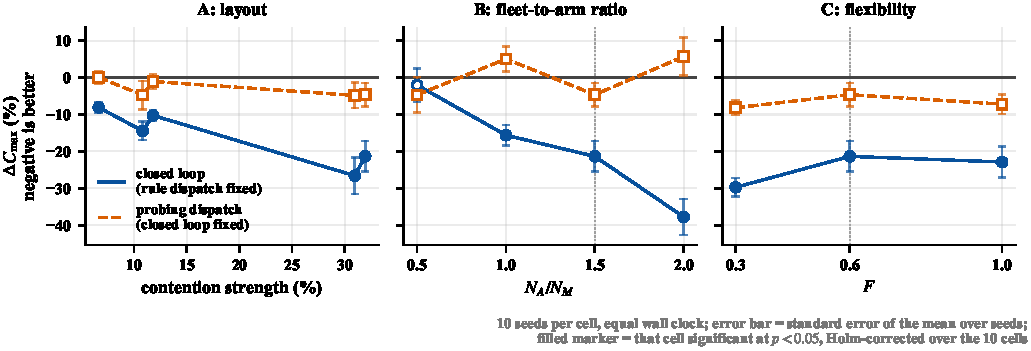
\includegraphics[width=\columnwidth]{fig/fig_prediction3.pdf}
\Description{Three panels of line plots: closed-loop gain and reservation-aware
dispatch gain across layout (vs contention), fleet-to-arm ratio, and flexibility. After
Holm correction over the ten cells the closed-loop curve is filled, hence
significant, at nine of ten cells, while the dispatch curve is hollow at every
cell, and its sign alternates across the four fleet-ratio levels. Error bars
give the standard error of the mean over the ten seeds of each cell; the
dispatch bars cross zero at every cell and the closed-loop bars do not.}
\caption{Closed-loop and dispatching gains by family: layout against contention intensity (left), $N_A/N_M$ (middle), flexibility (right); vertical lines mark the base point \texttt{A funnel}.
Filled markers: significant after Holm correction over the $\NCases$ instances of one effect. Error bars: standard error over $\NSeeds$ seeds.}
\label{fig:prediction3}
%% 由 fig/fig_prediction3_CN.py 从 clbs/output/baseline_ladder.csv 生成。横轴:A 族取争用强度
%% (布局族没有自然的数值水平,而布局操纵改变的正是争用),B/C 族取算例名末尾的因子水平——
%% 那个数字由 tools/abc_matrix.py 生成算例时写入,故按构造即为水平本身;基点 A funnel 的
%% 名字里没有水平,其 (1.5, 0.6) 由脚本按 abc_matrix.BASE 显式补入,见脚本内注释。
%% 标记的实心/空心由逐格 Wilcoxon 的 p 值决定。上一版按增益是否为正标注 "harmful",
%% 那等于把不显著的符号当成结论,现已改为按显著性区分标记。
%% 2026-08-20:填充判据改为 Holm 校正后的 p 值,族取该效应的全部十格(而不是当前面板的
%% 三到五格,否则共用基点会因所在面板不同而得到两种填充)。改动后试探那条曲线全为空心。
\end{figure}

In the layout family the closed loop is significant on all five instances and rises roughly with contention, from \GainLoopScatter{} on \texttt{scatter} (\ContentionLo{}) through \GainLoopMid{}/\GainLoopLow{} on \texttt{mid}/\texttt{low} to \GainLoopFunnel{}/\GainLoopHigh{} on \texttt{funnel}/\texttt{high}.
Two inversions qualify this: \texttt{low} versus \texttt{mid} straddles the topological boundary, but \texttt{funnel} versus \texttt{high} is the planned single-factor contrast, so \emph{this inversion is a counter-example}.
What is established is the magnitude, about two and a half times larger on the most congested instance than on the least, not a monotone relation between contention and gain; contention intensity does not separate the congestion that reassignment can bypass (Limitation~(1), Section~\ref{sec:limitations}).
Dispatching is significant on no instance here; four of five signs match the closed loop.

The vehicle-to-arm-ratio family does not establish an upper bound for dispatching: from $N_A/N_M=0.5$ to $2.0$ it is $-\GainProbeStarve$, \GainProbeFleetOne{}, \GainProbeFleetBase{}, and \GainProbeFleetTwo{}, alternating in sign and non-significant even before correction ($p\PProbeFleetHalfRaw$, $p\PProbeFleetOneRaw$, $p\PProbeFleetBaseRaw$, $p\PProbeFleetTwoRaw$).
Without the base point the curve would show the rise predicted by the cost law, so the upper bound of Section~\ref{sec:costlaw} remains untested; testing it needs more seeds than our budget allows.
The closed loop stays significant at $1.0$ and $2.0$ (\GainLoopFleetOne{}, \GainLoopFleetTwo{}): fleet size mainly affects the closed-loop gain.

In the flexibility family dispatching is \GainProbeFlexLo{}, \GainProbeFleetBase{}, and \GainProbeFlexHi{}, all with the pooled sign; the two ends are the largest magnitudes but lose significance after correction.
Since $F=0.3$, with the least room for reassignment, has the largest magnitude, dispatching appears to act through vehicle selection and timing rather than reassignment.
The closed loop is \GainLoopFlexLo{} and \GainLoopFlexHi{}, significant after correction.

\paragraph{Independent batch and heterogeneity.}
A separate batch of contended self-generated instances ($\MatrixRuns$ runs; Table~\ref{tab:batches}) crosses four contention levels with four $H$ levels against a two-stage surrogate-transport baseline.
Its \emph{integration gain} (two-stage $\to$ closed loop), \GainIntegMatrix{}, significant on \SigIntegMatrix{} instances (uncorrected), matches the closed loop here in direction and magnitude.
By $H$ level it is \GainIntegHZero{} at $H=0$, \GainIntegHLow{} at $0.15$ (measured \MatrixHMeasLow{}, near the public median \PubHMed{}), \GainIntegHMid{} at $0.3$, and \GainIntegHHigh{} at $0.5$, with a weakly negative rank correlation \RhoIntegH{}.
Setting $H$ above the literature range thus did not raise the gain; with four instances per level and a within-level spread (\GainIntegMatrixLo{} to \GainIntegMatrixHi{}) far exceeding the gaps between levels, the data support only that the gain does not rise with $H$, not that $H=0.5$ is lower.
As Section~\ref{sec:features} predicts, a larger $H$ lets processing speed rather than traffic decide assignment, while $H=0$ makes reassignment a pure congestion decision and has the highest gain; $H$ creates the trade-off behind the reversal of Section~\ref{sec:Chapter_I} but does not amplify the closed-loop gain.
For dispatching this batch gives \GainProbePre{} ($0$ instances significant), opposite to the main batch; it ran before the two speed-ups (Section~\ref{sec:costlaw}).
